\documentclass[12pt,oneside]{article}
%\usepackage[a4paper, left=2.5cm, right=2.5cm, top=2.5cm, bottom=1in]{geometry}
\usepackage[a4paper]{geometry}

\usepackage{amsmath}
\usepackage{amssymb}
\usepackage{amstext}
\usepackage{amsthm}

% for bibliography:
%\usepackage{comment}
%\usepackage[ backend=biber, style=chicago ]{biblatex}
%\usepackage[
%backend=biber,
%style=numeric,
%]{biblatex}
%\DeclareNameAlias{default}{last-first}

%\addbibresource{biblio.bib}
% see:
% https://www.sharelatex.com/learn/Bibliography_management_in_LaTeX#The_bibliography_file

\usepackage[export]{adjustbox}
\usepackage{tikz}
\usetikzlibrary{arrows}
\usetikzlibrary{scopes}
\usetikzlibrary{babel}

% For cross references
%\usepackage{hyperref}
\usepackage[colorlinks = true]{hyperref}
\usepackage[catalan]{varioref}
%\usepackage{cleveref}
%hyperref configuration so that it doesn't contrast so much colorlinks,
\usepackage{xcolor}
\hypersetup{
   linkcolor={black},
   citecolor={black},
   %linkcolor={red!50!black},
   %citecolor={blue!50!black},
   urlcolor={blue!80!black} }

% Custom Math operators (functions not in italic in math mode):
\DeclareMathOperator{\arcsec}{arcsec}
\DeclareMathOperator{\arccot}{arccot}
\DeclareMathOperator{\arccsc}{arccsc}
\DeclareMathOperator{\cis}{cis}

\usepackage[spanish]{babel} %Names in spanish
\usepackage[utf8]{inputenc} %Use unicode
\usepackage[T1]{fontenc}
\usepackage{csquotes} %For bibliography quotations
%\DeclareQuoteAlias{spanish}{catalan}

\usepackage{array}
\usepackage{float}  %Force tables and images position (H and H!)
\usepackage{wrapfig} %Wrap images like in HTML
\usepackage{listings} %For code blocks
\usepackage{color}  %Custom colors for syntax highlight in listings

\usepackage{tabularx,colortbl, booktabs} %Better tables
\usepackage[alsoload=hep]{siunitx} %Better tables and SI units and uncertainties
\usepackage{longtable}
\sisetup{separate-uncertainty=true}
\sisetup{locale = FR} %commas and so on for spanish
\sisetup{
  per-mode=fraction,
  fraction-function=\nicefrac
}
\usepackage{multirow}
\usepackage{multicol}
\usepackage{makecell}%Slit cell in lines and more formating options inside table

\usepackage{datetime} %To customize date

\newdateformat{monthyeardate}{%
    \monthname[\THEMONTH], \THEYEAR}
%Now \monthyeardate\today gives the date without the day

\usepackage[framemethod=tikz]{mdframed}
\usepackage{nicefrac} %nice fractions in one line

%Subfigures
\usepackage{subcaption}
\usepackage{relsize} %Bigger math with mathlarger{___}

\usepackage[bottom]{footmisc} %footnote at the bottom

%\usepackage{multicol}

%\definecolor{codegreen}{rgb}{0,0.6,0} 
%\definecolor{codegray}{rgb}{0.5,0.5,0.5}
%\definecolor{codepurple}{rgb}{0.58,0,0.82}
%\definecolor{backcolour}{rgb}{0.95,0.95,0.92}

%\lstdefinestyle{mystyle}{ backgroundcolor=\color{backcolour},
    %commentstyle=\color{codegreen}, keywordstyle=\color{blue},
    %numberstyle=\tiny\color{codegray}, stringstyle=\color{red},
    %identifierstyle=\color{black}, basicstyle=\footnotesize,
    %%breakatwhitespace=false,         
    %breaklines=true,                 
    %%captionpos=b,                    keepspaces=true,                 
    %numbers=left,                    numbersep=5pt,
    %showspaces=false,                
    %%showstringspaces=false, showtabs=false,                  
    %tabsize=4 }

%\lstset{style=mystyle}


%%\renewcommand{\figurename}{Fig.} \renewcommand{\tablename}{Tabla}
%%tabla-es in babel better

%\definecolor{lightblue}{RGB}{135,206,250}

%% Add command before appendix session for page numbering: A-1
%\newcommand{\appendixpagenumbering}{
    %\break
    %\pagenumbering{arabic}
    %\renewcommand{\thepage}{\thesection-\arabic{page}}
%}

%\newcommand{\whitepage}{
    %\clearpage\thispagestyle{empty}\addtocounter{page}{-1} \newpage \clearpage
%}



\geometry{margin=1in}

\title{
   Probabilidad y estadística - B7 \\
   \large 
   - Estudio del oleaje y el viento en Nazaré y Jaws -
}
\author{
  Aleix Boné \and
  Alex Herrero \and
  Albert Mercadé
}
\date{
  \today
}

\begin{document}
\maketitle
%\tableofcontents

\begin{abstract}
% resumen
% <= 250 palabras
\end{abstract}

\section{Introducción}%
\label{sec:introduccion}
% Justificación + objetivos + hipotesis
El gran interés de uno de los integrantes del grupo, Alex Herrero, en el mundo del surf nos ha llevado a investigar este apasionante tema y nos ha introducido al resto del grupo al mundo del surf y la oceanografía. Dentro del ámbito del surf hay muchos factores a tener en cuenta en cuanto a lo que se refiere a la ``ola perfecta''. Entre ellos, dos de los más importantes son el tamaño de la ola y la velocidad del viento. Es un tema complejo dado que los datos que vamos a estudiar se ven afectados por muchos otros factores; la marea, el \textit{fetch}\footnote{La longitud rectilínea máxima de una gran masa de agua superficial que es uniformemente afectada por la dirección y fuerza del viento} o la complexión del fondo marino litoral.

En este caso queremos comparar dos de los \textit{surf spots}\footnote{Lugar con olas surfeables} más famosos y con las olas más grandes del mundo a lo largo de la historia; Nazaré en Portugal y Jaws en Peahi, Hawái. Paralelamente observaremos qué relación tiene la velocidad de viento con el tamaño de las olas en ambos sitios.

Nuestra hipótesis es que la media de la altura de las olas en Nazaré será superior a la de Jaws, dado que en los últimos años el récord de ola más grandes surfeada por el hombre se ha roto en Nazaré varias veces. Además, el fondo marino de Nazaré tiene un relieve mejor para la creación de olas gigantes. En cuanto a la relación entre la velocidad del viento y la altura de las olas, esperamos que la correlación sea positiva
puesto que la velocidad del viento es uno de los factores más importantes en la creación de las olas.

\section{Recogida de datos}%
\label{sec:recogida_de_datos}
% Recogida de datos + seleccion de datos
Para realizar nuestro análisis recogimos datos de viento y altura de olas de
dos localizaciones distintas. Escogimos dos playas conocidas por sus buenas
olas para hacer surf: Nazaré, Portugal y Jaws en Peahi, Hawái.

Pudimos obtener datos de oleaje y viento del archivo histórico de \emph{WindGuru}\footnote{\url{https://www.windguru.cz/archive.php}}, un servicio especializado en previsiones del tiempo para windsurfistas y kitesurfistas basado en el modelo numérico GFS\footnote{\url{https://es.wikipedia.org/wiki/Global_Forecast_System}}. Con un \textit{script} de
Python\footnote{El código se puede ver en el anexo
  \ref{sec:codigo_extraccion_de_datos}} extrajimos datos de la altura de las
olas y viento en periodos de 3 horas de 2006 hasta hoy. En el caso de Nazaré
obtuvimos datos de 4377 días (35016 periodos de 3 horas) y en Jaws 3338 días
(26704 periodos de 3 horas).

Con el fin de simplificar los cálculos al hacer la prueba de hipótesis y la regresión lineal simple nos interesa reducir la cantidad de datos que utilizamos en nuestro estudio. Para ello, hemos decidido considerar solo los datos de entre las 8:00 y las 17:00 usando la función \texttt{subset} de R, debido a que la gran mayoría de surfistas practican el surf en esta franja horaria. Asimismo, hemos usado la función \texttt{sample\_n} de la librería \texttt{dplyr} de R para reducir aleatoriamente aún más los datos de cada \textit{surf spot} hasta los 500 \textit{data points}. Usando estos criterios, hemos reducido la cantidad de datos para Nazaré y Jaws desde los 35016 y 26704 periodos respectivamente hasta los 500 para cada uno.

\section{Análisis Descriptivo}%
\label{sec:metodos}

\begin{table}[htbp]
    \centering
    \begin{tabular}{lS[table-format=1.3]S[table-format=2.3]}
    \toprule
    & {Altura Ola (\si{\meter})} & {Velocidad Viento (\si{\knot})} \\
    \midrule
    Min.   & 0.0&  0   \\ 
    1er Cu.& 1.6   &  5   \\ 
    Mediana & 2.1   &  8   \\ 
    Media   & 2.414   &  8.666   \\ 
    3er Cu.& 3.0   & 11   \\ 
    Máx.   &11.4   & 38   \\ 
    \bottomrule
\end{tabular}

    \caption{summary Nazaré}
    \label{tab:summary_nazare}
\end{table}

El Cuadro \ref{tab:summary_nazare} muestra un resumen de los datos recogidos sobre Nazaré. Cómo se puede observar la altura máxima registrada es de 11.4 metros, a pesar de ello la media es de 2.4 metros debido a que durante la mayoría de días la altura está cerca del mínimo (0 metros). Por este mismo motivo la mediana (de 2.1 metros) se encuentra por debajo de la media, y el primer y tercer cuartiles son de 1.6 y 3 metros respectivamente. Dicha distribución se puede ver con claridad en la Figura \ref{fig:hist_waves_nazare}.

\begin{figure}[H]
    \centering
    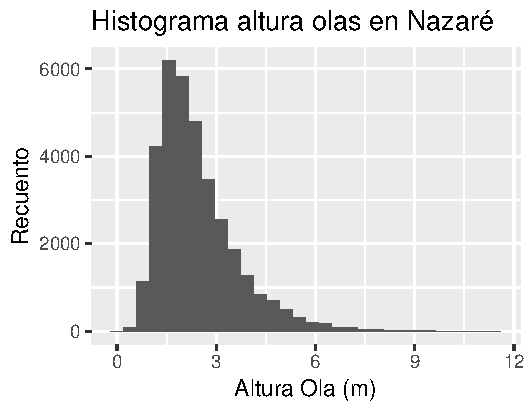
\includegraphics[height=5.6cm]{./figures/nazare_hist_wave.pdf}
    \caption{Histograma de olas en Nazaré}
    \label{fig:hist_waves_nazare}
\end{figure}

Con respecto a los datos sobre la velocidad del viento sucede algo parecido, pero en este caso los datos se concentran sobre todo entre la mediana (8 nudos) y el tercer cuartil (11 nudos) ya que la media es de 8.6 nudos. Sin embargo el valor máximo se aleja mucho de la media llegando a multiplicar su valor por más de cuatro siendo este de 38 nudos. También se puede observar que el mínimo, al igual que con la altura es de 0 nudos.


\begin{table}[htbp]
    \centering
    \begin{tabular}{lS[table-format=1.3]S[table-format=2.3]}
    \toprule
    & {Altura Ola (\si{\meter})} & {Velocidad Viento (\si{\knot})} \\
    \midrule
    Min.    &0.0      &  0    \\
    1er Cu.  &1.6    &  8    \\
    Mediana &1.9    & 12    \\
    Media   &2.047  & 11.46 \\
    3er Cu.  &2.4    & 15    \\
    Máx.    &5.9    & 32    \\
    \bottomrule
\end{tabular}

    \caption{summary Jaws}
    \label{tab:summary_jaws}
\end{table}


En el caso de Jaws, los datos se exponen en el Cuadro \ref{tab:summary_jaws}, y se observa que la distribución de la altura es bastante similar a la de Nazaré pero los datos están levemente más centrados (véase Figura \ref{fig:hist_waves_jaws}). En Jaws el rango de altura es menor ya que el valor mínimo sigue siendo de 0 metros pero el máximo en cambio es de 5.9, casi la mitad que en Nazaré. La media y la mediana prácticamente coinciden siendo 2 y 1.9 metros respectivamente. El primer cuartil se encuentra en 1.6 metros y el tercero en 2.4 metros.

\begin{figure}[H]
    \centering
    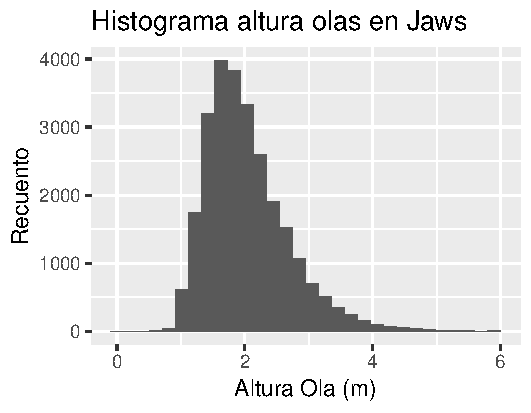
\includegraphics[height=5.6cm]{./figures/jaws_hist_wave.pdf}
    \caption{Histograma de olas en Jaws}
    \label{fig:hist_waves_jaws}
\end{figure}

La velocidad del viento en Jaws en comparación con la de Nazaré, a pesar de que el máximo (32 nudos) es inferior, es mucho superior con una media de 11.4 \si{\knot}. Tiene una distribución relativamente simétrica ya que la mediana se encuentra en 12 nudos y el primer y tercer cuartiles en 8 y 15 nudos respectivamente. El mínimo como es de esperar también es de 0 nudos.

\begin{figure}[H]
    \begin{subfigure}{.49\textwidth}
        \centering
        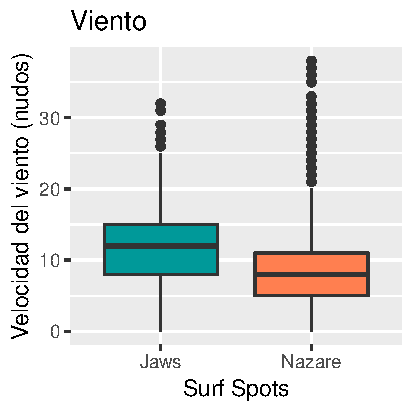
\includegraphics[width=0.9\textwidth]{./figures/boxplot_wind.pdf}
        \caption{Boxplot Viento}
        \label{fig:boxplot_wind}
    \end{subfigure}%
    \begin{subfigure}{.49\textwidth}
        \centering
        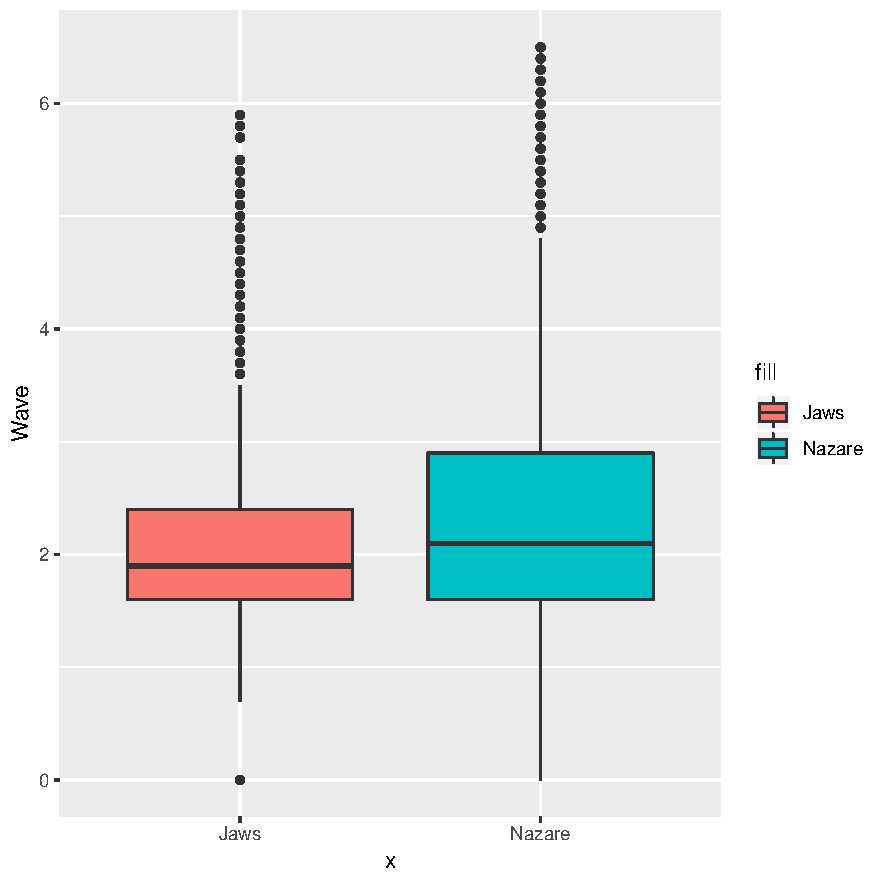
\includegraphics[width=0.9\textwidth]{./figures/boxplot_wave.pdf}
        \caption{Boxplot Olas}
        \label{fig:boxplot_wave}
    \end{subfigure}
    \caption{Boxplots}
    \label{fig:boxplots}
\end{figure}

En la Figura \ref{fig:boxplot_wind} podemos ver claramente como la media de la velocidad del viento en Jaws es superior a la de Nazaré, no obstante la variabilidad de Jaws es ligeramente superior como se puede apreciar en el primer cuartil. En cuanto a la altura de las olas (véase Figura \ref{fig:boxplot_wave}), la media es levemente mayor y a diferencia del viento, en este caso es Nazaré que tiene una variación ostensiblemente más amplia.

\section{Análisis Inferencial}%
\label{sec:resultados}
% Descriptiva más inferencia

\section{Análisis de Regresión Lineal Simple}
\label{sec:rls}

\begin{figure}[H]
    \centering
    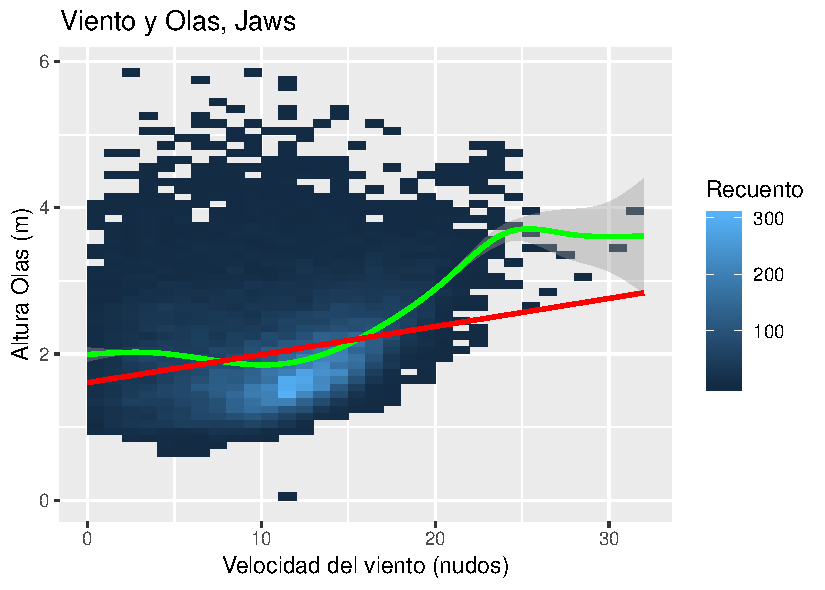
\includegraphics{./figures/jaws_all.pdf}
    \caption{Velocidad de viento vs. Altura de olas en Jaws en Peahi, Hawái}
    \label{fig:wind_waves_jaws_all}
\end{figure}

\begin{figure}[H]
    \centering
    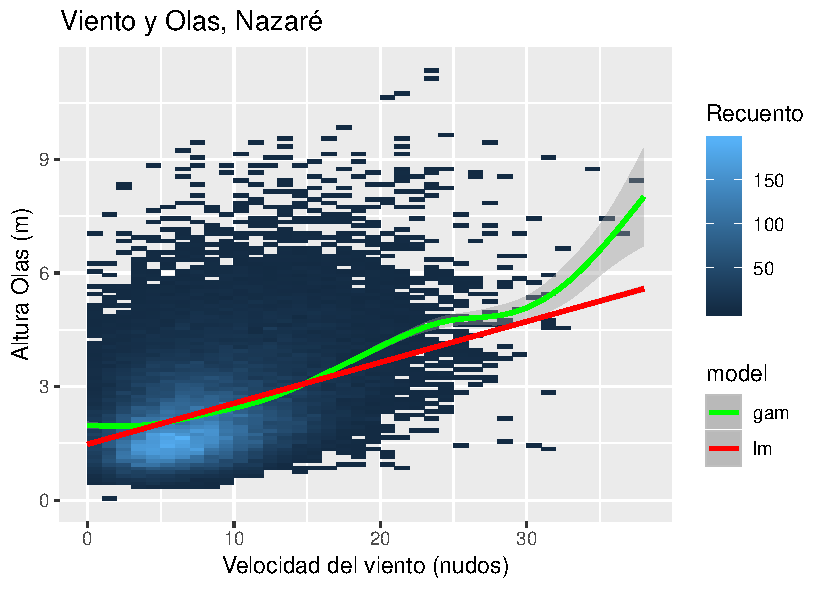
\includegraphics{./figures/nazare_all.pdf}
    \caption{Velocidad de viento vs. Altura de olas en Nazaré, Portugal}
    \label{fig:wind_waves_nazare_all}
\end{figure}

%\begin{figure}[H]
%    \centering
%    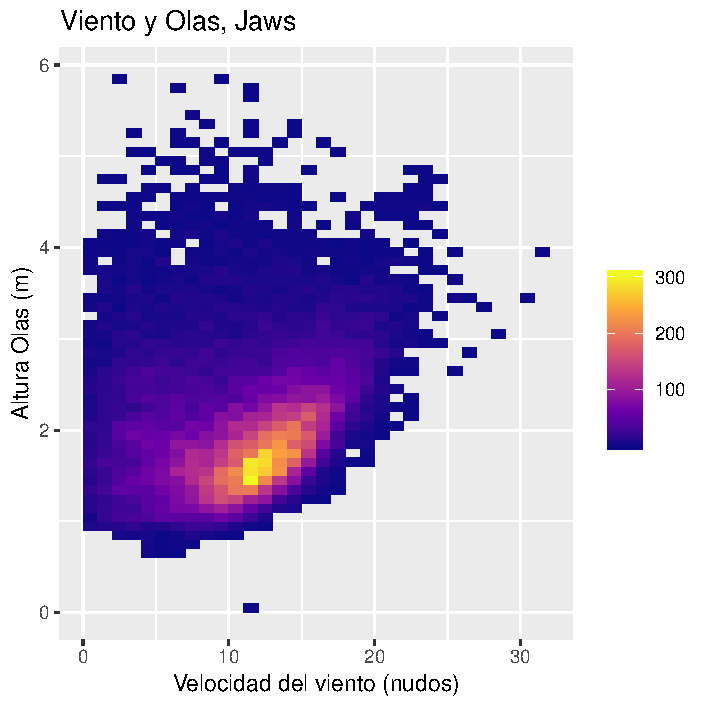
\includegraphics[width=0.6\textwidth]{./figures/jaws_bin2d.pdf}
%    \caption{Velocidad de viento vs. Altura de olas en Jaws en Peahi, Hawái}
%    \label{fig:wind_waves_jaws}
%\end{figure}
%
%\begin{figure}[H]
%    \centering
%    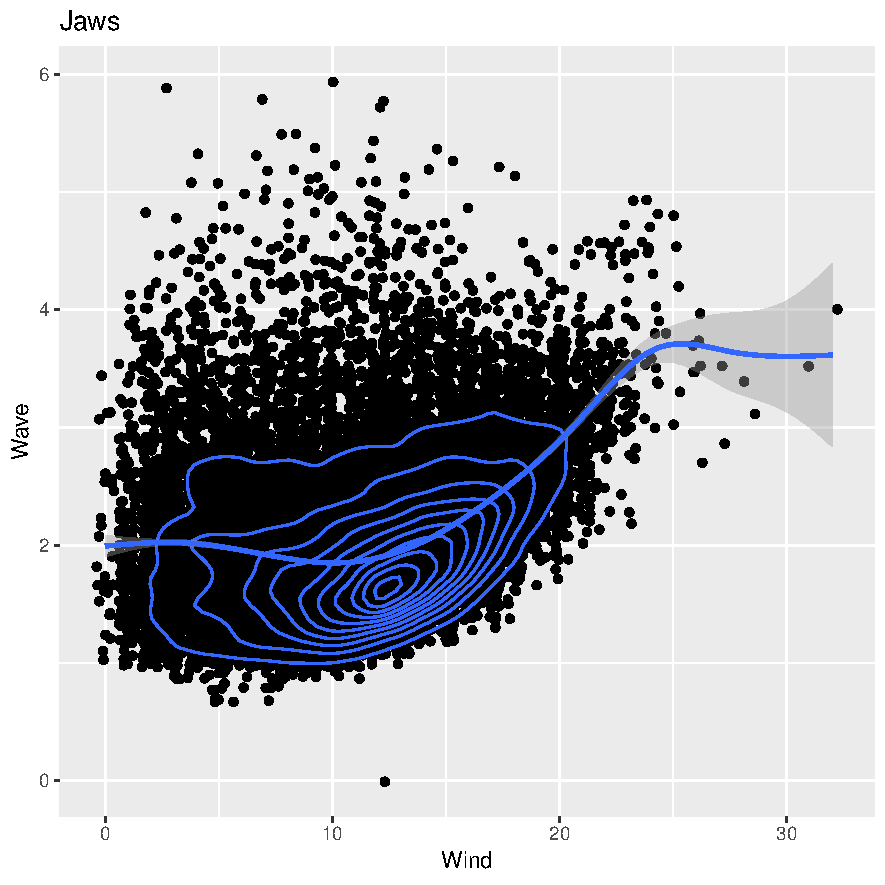
\includegraphics[width=0.6\textwidth]{./figures/jaws_smooth.pdf}
%    \caption{Velocidad de viento vs. Altura de olas en Jaws en Peahi, Hawái}
%    \label{fig:jaws_smooth}
%\end{figure}
%
%\begin{figure}[H]
%    \centering
%    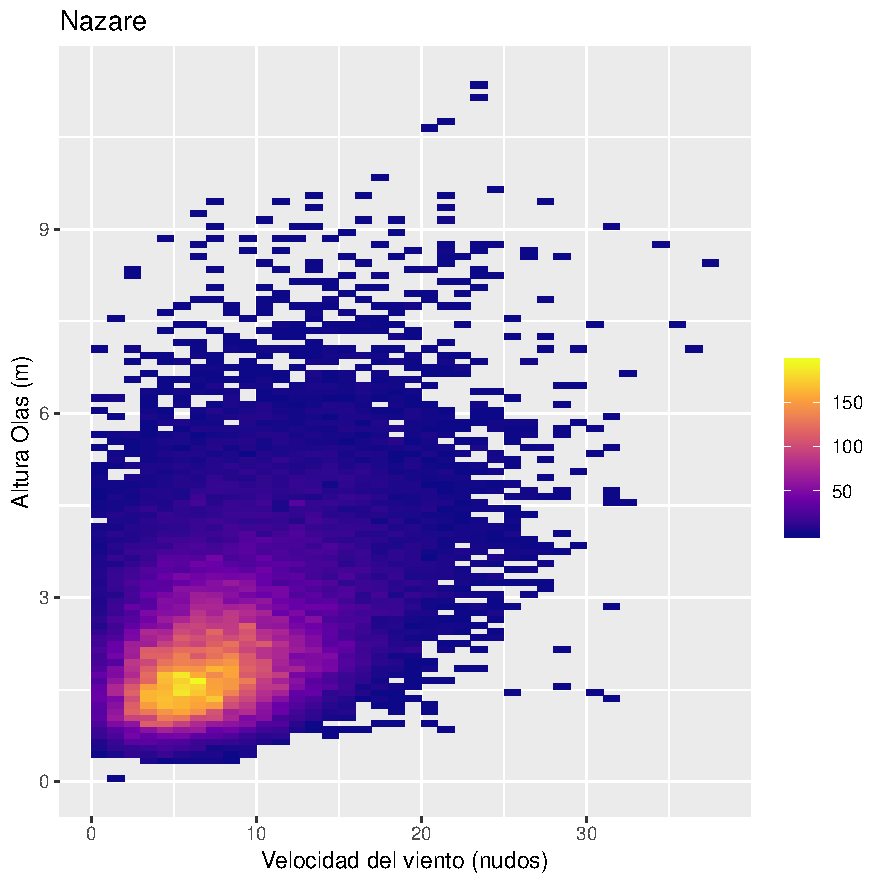
\includegraphics[width=0.6\textwidth]{./figures/nazare_bin2d.pdf}
%    \caption{Velocidad de viento vs. Altura de olas en Nazaré, Portugal}
%    \label{fig:wind_waves_nazare}
%\end{figure}
%
%\begin{figure}[H]
%    \centering
%    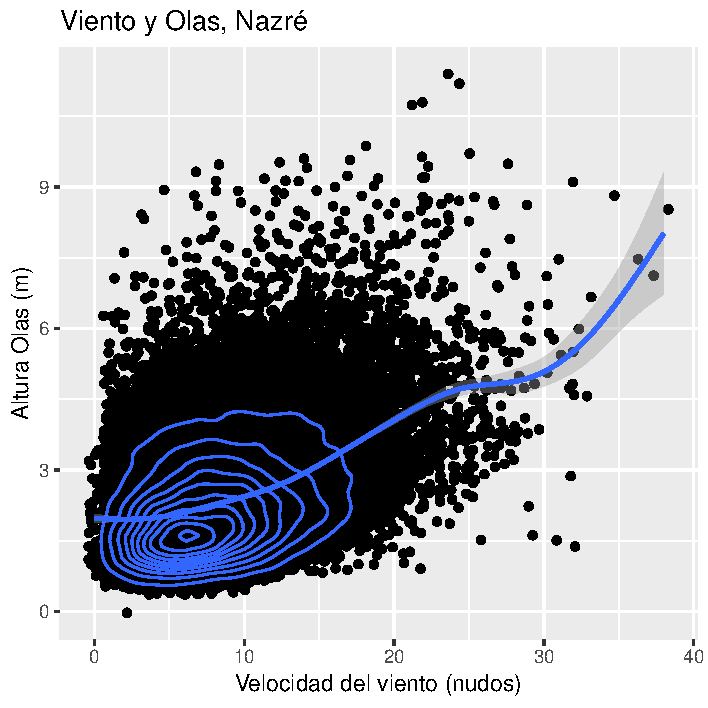
\includegraphics[width=0.6\textwidth]{./figures/nazare_smooth.pdf}
%    \caption{Velocidad de viento vs. Altura de olas en Nazaré, Portugal}
%    \label{fig:nazare_smooth}
%\end{figure}

\section{Discusión}%
\label{sec:discusión}

\pagebreak
\appendix

\section{Código extracción de datos}%
\label{sec:codigo_extraccion_de_datos}

\lstinputlisting[language=Python]{./process.py}
\end{document}

% vim:sw=2:ts=2:et:spell:spelllang=es: